\subsection{Architektura knihovny}

Filozofie architektury za \texttt{framesss} spočívá v tvorbě robustního a flexibilního systému schopného přizpůsobit se aktuálním i budoucím potřebám. Tento přístup byl klíčový při formování modulárního designu softwaru, který umožňuje aktualizaci nebo výměnu jednotlivých komponent bez dopadu na celkový systém. Objektově orientovaný design podporuje tuto modularitu, což zvyšuje opětovnou použitelnost kódu a udržitelnost.

\subsubsection{Funkce programu}

Knihovna \texttt{framesss} je vybavena následující funkčností:

\begin{itemize}
    \item \textbf{Typy modelů}: V současné době knihovna podporuje pouze 2D statický výpočet rámu v rovině \gls{X}\gls{Z}, plánuje se rozšíření na 3D modely.
    \item \textbf{Typ výpočtu}: Lineárně pružná statická analýza.
    \item \textbf{Podpory}: 
        \begin{itemize}
            \item \textbf{Pevné}: Kompletně zabraňují posunu nebo pootočení v daném směru.
            \item \textbf{Pružné}: Podpora je v daném směru pružná, uživatel musí zadat tuhost podepření.
        \end{itemize}
    \item \textbf{Typy prutů}:
        \begin{itemize}
            \item \textbf{Navier (Euler-Bernoulli)}: Průřezy po deformaci zůstavají kolmé na deformovanou střednici prutu,
            \item \textbf{Timoshenko}: Průřez po deformaci zůstává rovinný, ale ne nutně kolmý na deformovanou střednici prutu.
        \end{itemize}
    \item \textbf{Zatížení}:
        \begin{itemize}
            \item \textbf{Silová zatížení}: Uzlové síly a momenty, osamělé síly a momenty na prvcích, rovnoměrná a lineární spojitá zatížení působící na celé délce nebo jen části prutu. Zatížení na prvcích mohou působit v globálním souřadném systému nebo v lokálním systému prutu. Spojitá zatížení v globálním souřadném systému lze zadávat jako působící na délku nebo na průmět prvku, viz obr. \ref{fig:distributed_load}.
            \item \textbf{Předepsané deformace uzlů}: Tento typ zatížení lze zadat pouze v podepřených uzlech.
            \item \textbf{Zatížení teplotou}: Lze zadat zatížení rovnoměrnou nebo nerovnoměrnou změnou teplot na celém prvku.
        \end{itemize}
    \item \textbf{Zatěžovací stavy}: Jednotlivá zatížení lze sloučit do zatěžovacích stavů.
    \item \textbf{Kombinace zatížení}: Více zatěžovacích stavů může být kombinováno s uplatněním kombinačních součinitelů.
    \item \textbf{Obálka}: Kombinuje různé kombinace zatížení pro získání obálky výsledků s maximální a minimální odezvou.
\end{itemize}

\begin{figure}[H]
    \begin{tikzpicture}
    \scaling{1}
    \point{a}{0}{0}
    \point{b}{3}{2}
    \beam{1}{a}{b}
    \lineload{3}{a}{b}[0.7][0.7][2]
    
    \point{c}{3.5}{0}
    \point{d}{6.5}{2}
    \beam{1}{c}{d}
    \lineload{2}{c}{d}[0.7][0.7]

    \point{e}{7}{0}
    \point{f}{10}{2}
    \beam{1}{e}{f}
    \lineload{1}{e}{f}[0.7][0.7]
\end{tikzpicture}
    \caption{Typy spojitého zatížení}
    \label{fig:distributed_load}
\end{figure}

\texttt{framesss} je strukturován do čtyř základních modulů, které společně zajišťují celý proces statického výpočtu. Tyto moduly jsou:
\begin{itemize}
    \item \textbf{\texttt{pre}},
    \item \textbf{\texttt{fea}},
    \item \textbf{\texttt{solvers}},
    \item \textbf{\texttt{post}}.
\end{itemize}

%%%%%%%%%%%%%%%%%%%%%%%%%%%%%%%%%%%%%%%% PRE %%%%%%%%%%%%%%%%%%%%%%%%%%%%%%%%%%%%%%%%%%%%%%%

\subsubsection*{Modul \texttt{pre}}
Modul zodpovídá za přípravu a definici vstupních dat modelu. Uživatelé zde mohou definovat geometrii, materiály, zatížení a podpory. Jedná se o klíčový modul, který umožňuje definici modelu před spuštěním vlastního výpočtu.

Na obr. \ref{fig:modul_pre} je diagram hierarchie tříd v modulu 
\href{https://danberanek.github.io/framesss/gen/framesss.pre.cases.html#module-framesss.pre.cases}{\texttt{pre}}.
Třídy v tomto modulu se starají o přípravu a definici vstupních dat modelu. V diagramu vidíme třídu pro průřezy 
\href{https://danberanek.github.io/framesss/gen/framesss.pre.section.Section.html#framesss.pre.section.Section}{\texttt{Section}}
 a její konkrétní implementace 
 \href{https://danberanek.github.io/framesss/gen/framesss.pre.section.RectangularSection.html#framesss.pre.section.RectangularSection}{\texttt{RectangularSection}} 
 a \href{https://danberanek.github.io/framesss/gen/framesss.pre.section.PolygonalSection.html#framesss.pre.section.PolygonalSection}{\texttt{PolygonalSection}}. Dále jsou zde třídy pro zatížení, jako 
 \href{https://danberanek.github.io/framesss/gen/framesss.pre.member_load.DistributedLoadOnMember.html#framesss.pre.member_load.DistributedLoadOnMember}{\texttt{DistributedLoadOnMember}}, 
 \href{https://danberanek.github.io/framesss/gen/framesss.pre.member_load.ThermalLoadOnMember.html}{\texttt{ThermalLoadOnMember}} a 
 \href{https://danberanek.github.io/framesss/gen/framesss.pre.member_load.PointLoadOnMember.html}{\texttt{PointLoadOnMember}}. 
 Modul také obsahuje třídu pro zatěžovací stavy 
 \href{https://danberanek.github.io/framesss/gen/framesss.pre.cases.LoadCase.html}{\texttt{LoadCase}}, jejich kombinace 
 \href{https://danberanek.github.io/framesss/gen/framesss.pre.cases.LoadCaseCombination.html}{\texttt{LoadCaseCombination}} a obálku výsledků 
 \href{https://danberanek.github.io/framesss/gen/framesss.pre.cases.EnvelopeCombination.html}{\texttt{EnvelopeCombination}}. Také je zde třída pro prutový prvek 
 \href{https://danberanek.github.io/framesss/gen/framesss.pre.member_1d.Member1D.html#framesss.pre.member_1d.Member1D}{\texttt{Member1D}} a třída pro materiál \href{https://danberanek.github.io/framesss/gen/framesss.pre.material.Material.html#framesss.pre.material.Material}{\texttt{Material}}.

\begin{figure}[H]
    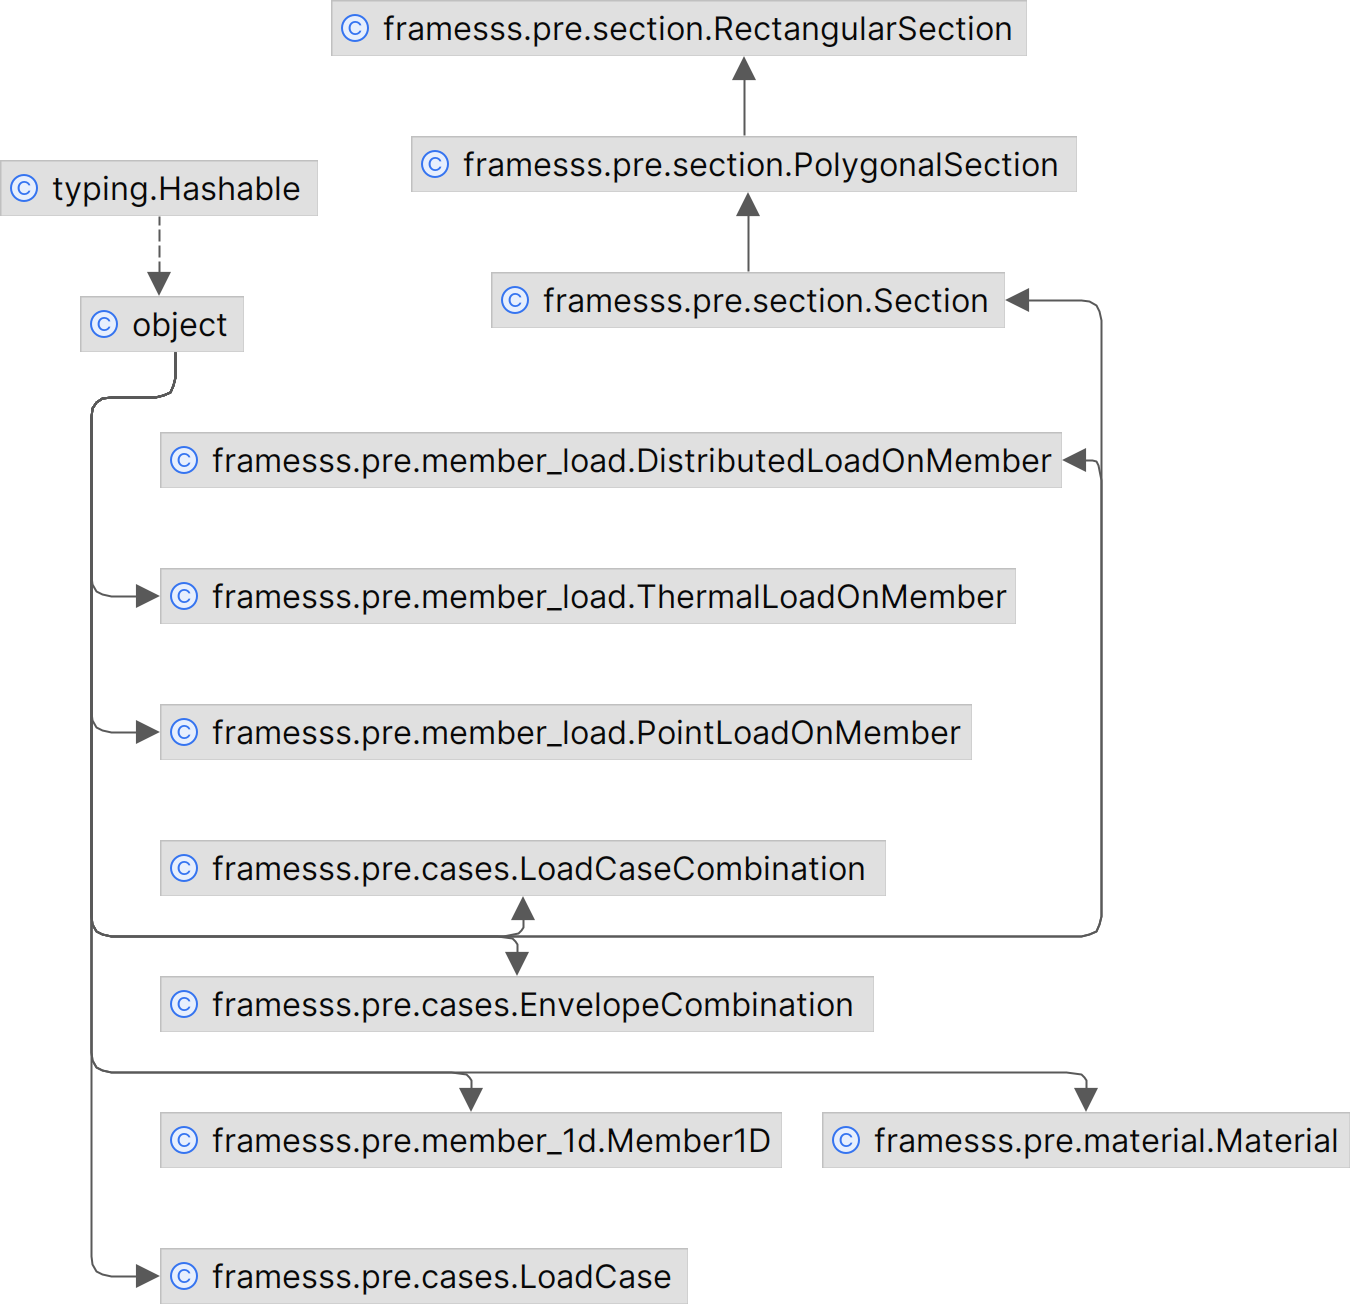
\includegraphics{assets/figures/framesss/uml/pre.png}
    \caption{Diagram modulu \texttt{pre}}
    \label{fig:modul_pre}
\end{figure}

%%%%%%%%%%%%%%%%%%%%%%%%%%%%%%%%%%%%%%%% FEA %%%%%%%%%%%%%%%%%%%%%%%%%%%%%%%%%%%%%%%%%%%%%%%

\subsubsection*{Modul \texttt{fea}}
Na obr. \ref{fig:modul_fea} je diagram zobrazující hierarchii tříd v modulu 
\href{https://danberanek.github.io/framesss/gen/framesss.fea.html}{\texttt{fea}}, který je srdcem knihovny \texttt{framesss}. Klíčovou třídou je
\href{https://danberanek.github.io/framesss/gen/framesss.fea.models.model.Model.html#framesss.fea.models.model.Model}{\texttt{Model}}, která je zodpovědná za přidávání prvků (uzly, prvky, zatěžovací stavy, zatížení atd.) a drží v sobě všechny instance, které se následně předávají do řešiče (solveru). Pod ní jsou specifické modely, jako
\href{https://danberanek.github.io/framesss/gen/framesss.fea.models.frame_xz.FrameXZModel.html#framesss.fea.models.frame_xz.FrameXZModel}{\texttt{FrameXZModel}}. Modul také obsahuje třídy pro definici elementů
\href{https://danberanek.github.io/framesss/gen/framesss.fea.element_1d.Element1D.html#framesss.fea.element_1d.Element1D}{\texttt{Element1D}}
 a uzlů
 \href{https://danberanek.github.io/framesss/gen/framesss.fea.node.Node.html#framesss.fea.node.Node}{ \texttt{Node}}. Pro zatížení elementů zde máme abstraktní třídu 
 \href{https://danberanek.github.io/framesss/gen/framesss.fea.boundary_conditions.element_load.ElementLoad.html#framesss.fea.boundary_conditions.element_load.ElementLoad}{\texttt{ElementLoad}}, ze které vychází třída pro zatížení spojitým zatížením
 \href{https://danberanek.github.io/framesss/gen/framesss.fea.boundary_conditions.element_load.DistributedLoad.html}{\texttt{DistributedLoad}}
 a třída pro zatížení teplotou
 \href{https://danberanek.github.io/framesss/gen/framesss.fea.boundary_conditions.element_load.ThermalLoad.html}{\texttt{ThermalLoad}}, dále je zde třída pro uzlové zatížení
 \href{https://danberanek.github.io/framesss/gen/framesss.fea.boundary_conditions.nodal_load.NodalLoad.html}{\texttt{NodalLoad}}, a pro předepsané přemístění podpor
\href{https://danberanek.github.io/framesss/gen/framesss.fea.boundary_conditions.prescribed_displacement.PrescribedDisplacement.html#framesss.fea.boundary_conditions.prescribed_displacement.PrescribedDisplacement}{ \texttt{PrescribedDisplacement}}.
 Modul také zahrnuje třídy pro specifikování dimenze problému, které vychází z abstraktní třídy
 \href{https://danberanek.github.io/framesss/gen/framesss.fea.analysis.analysis.Analysis.html#framesss.fea.analysis.analysis.Analysis}{\texttt{Analysis}}
 a její konkrétní implementace pro různé typy konstrukcí, např.
 \href{https://danberanek.github.io/framesss/gen/framesss.fea.analysis.frame_xz_analysis.FrameXZAnalysis.html#framesss.fea.analysis.frame_xz_analysis.FrameXZAnalysis}{\texttt{FrameXZAnalysis}}.

\begin{figure}[H]
    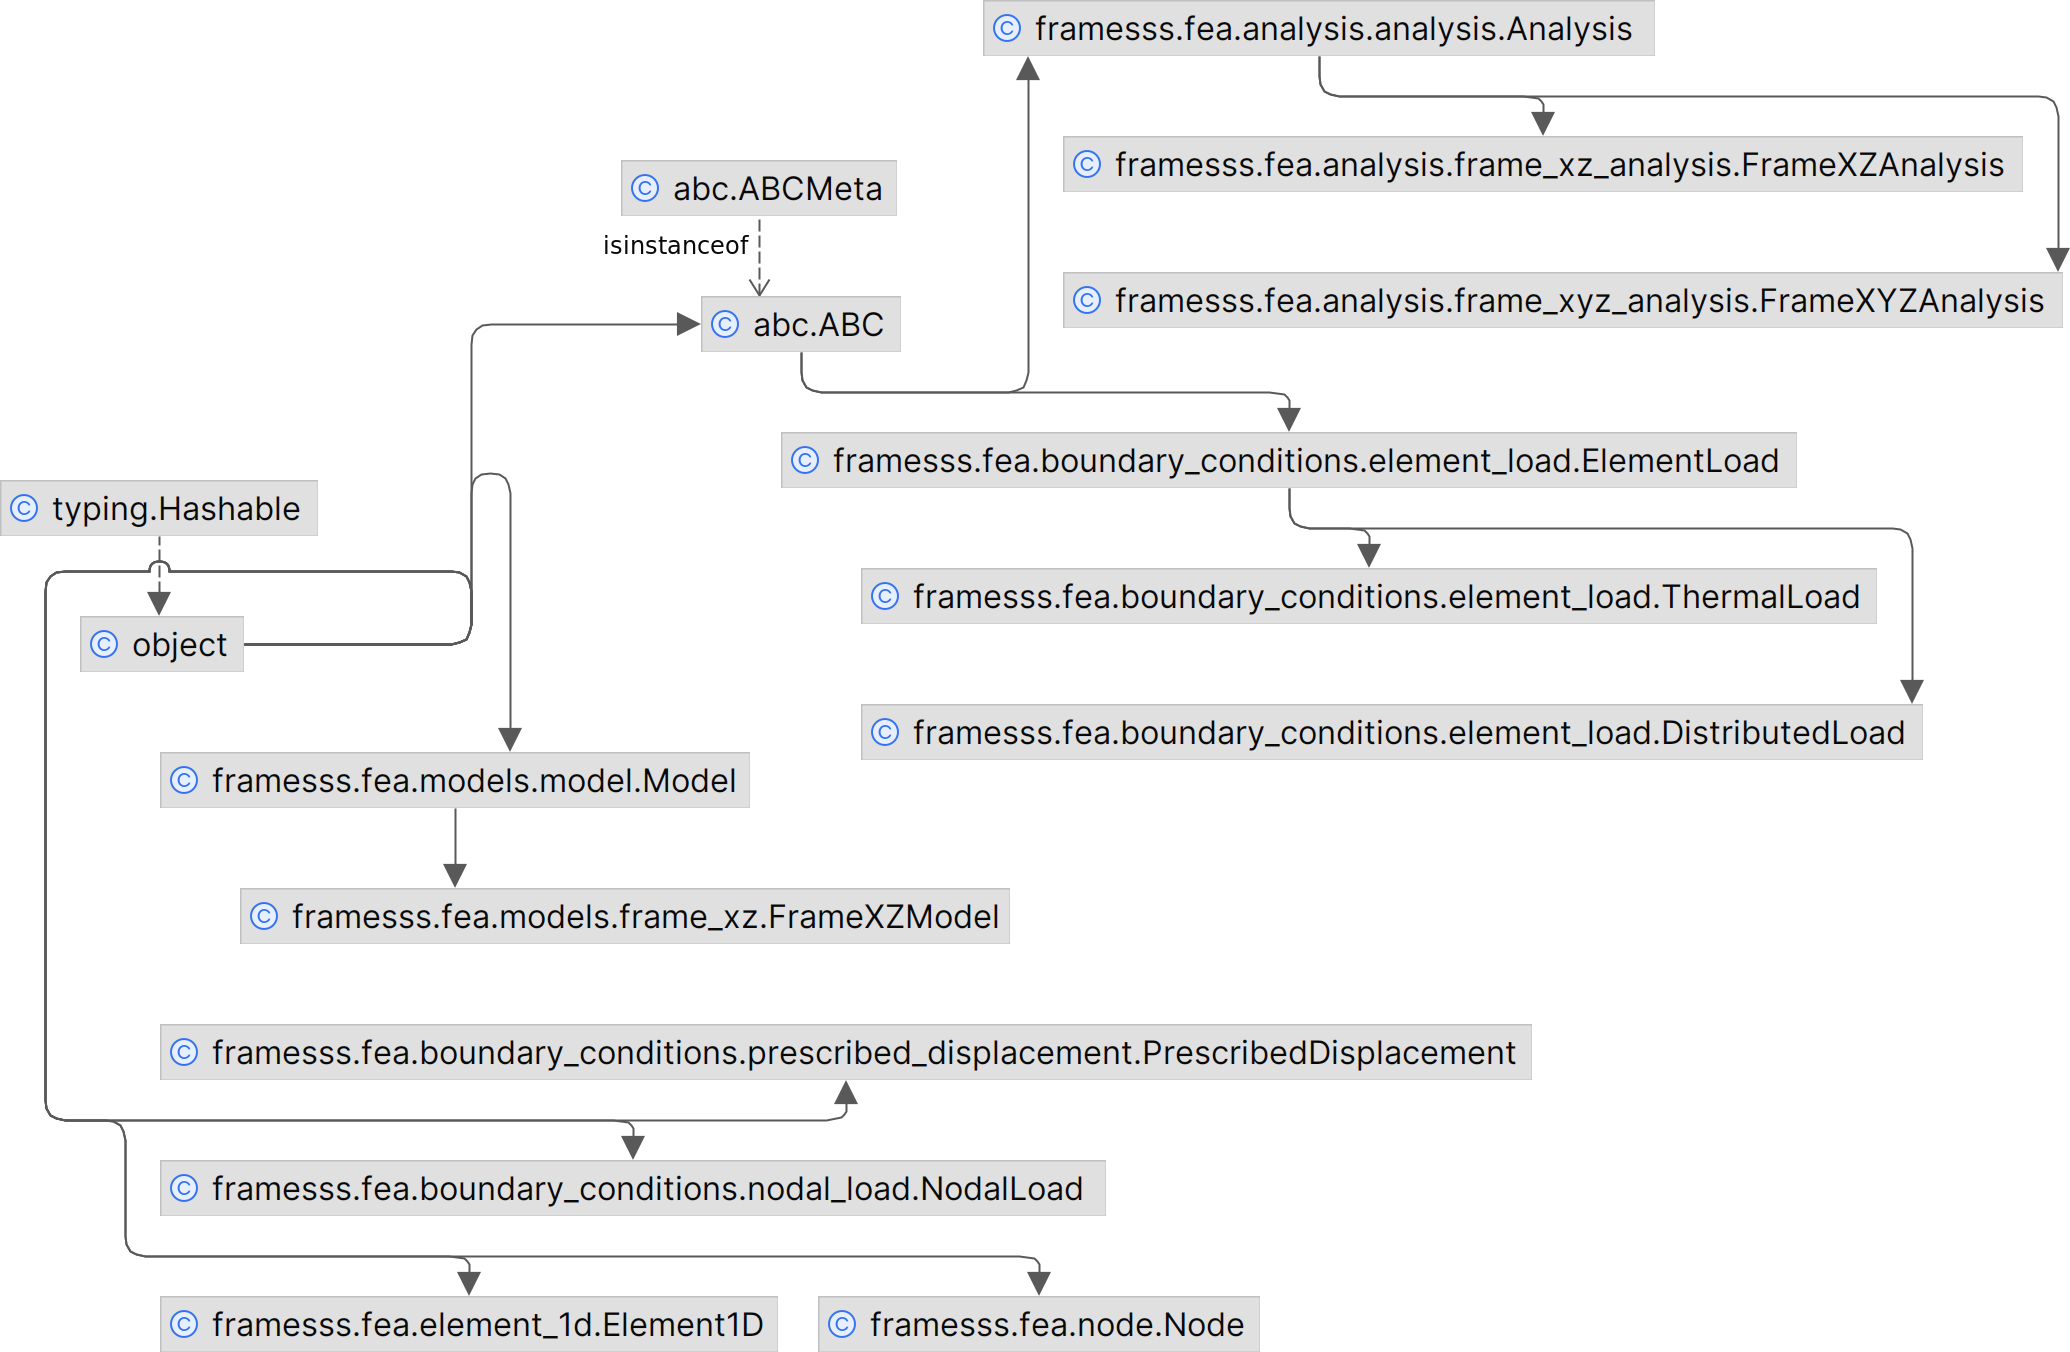
\includegraphics{assets/figures/framesss/uml/fea.png}
    \caption{Diagram modulu \texttt{fea}}
    \label{fig:modul_fea}
\end{figure}

\subsubsection*{Modul \texttt{solvers}}
Modul obsahuje řešiče používané pro výpočty v modulu
\href{https://danberanek.github.io/framesss/gen/framesss.fea.html}{\texttt{fea}}. Na  obr. \ref{fig:modul_solvers} je znázorněný diagram hierarchie tříd v modulu
\href{https://danberanek.github.io/framesss/gen/framesss.solvers.html}{\texttt{solvers}}. Základem této hierarchie je třída \texttt{abc.ABC}, což je základní abstraktní třída v Pythonu. Na jejím základě je definována třída
\href{https://danberanek.github.io/framesss/gen/framesss.solvers.solver.Solver.html}{\texttt{Solver}}, která slouží jako základ pro konkrétní implementace řešičů. Jediným implementovaným řešičem je v současné době třída
\href{https://danberanek.github.io/framesss/gen/framesss.solvers.linear_static.LinearStaticSolver.html}{\texttt{LinearStaticSolver}}, která implementuje lineární statické výpočty.

\begin{figure}[H]
    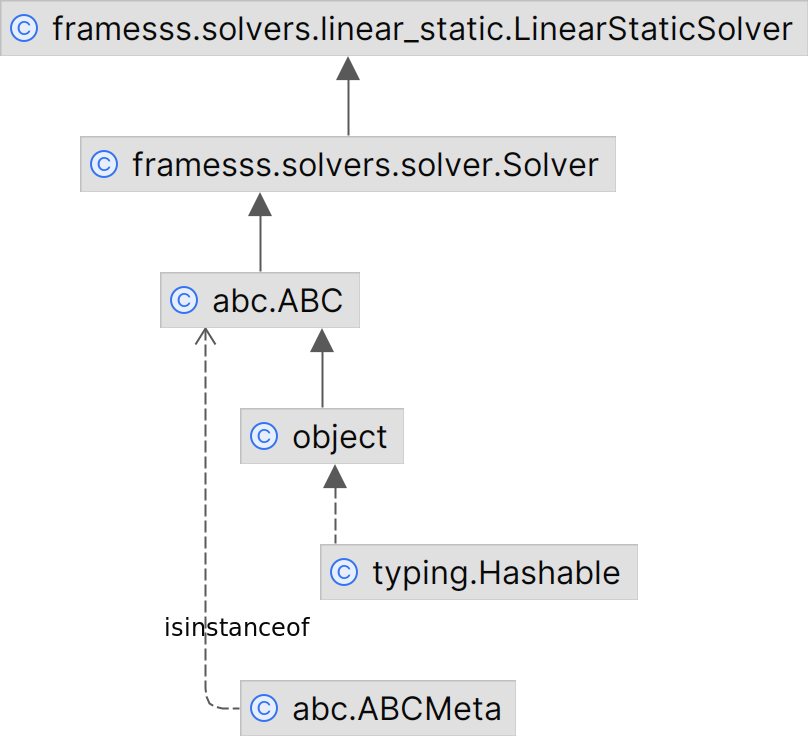
\includegraphics{assets/figures/framesss/uml/solvers.png}
    \caption{Diagram modulu \texttt{solvers}}
    \label{fig:modul_solvers}
\end{figure}

\subsubsection*{Modul \texttt{post}}
Zpracovává výsledky, jako jsou posuny a vnitřní síly, které jsou získány z výpočtu provedených modulem \href{https://danberanek.github.io/framesss/gen/framesss.fea.html}{\texttt{fea}}. Modul nezahrnuje vizualizaci, ale umožňuje uživatelům extrahovat a prohlížet vypočítané hodnoty, které mohou být dále použity.
Diagram na obr. \ref{fig:modul_post} ukazuje hierarchii tříd v modulu \href{https://danberanek.github.io/framesss/gen/framesss.post.html}{\texttt{post}}, který je zodpovědný za zpracování výsledků. Třída 
\href{https://danberanek.github.io/framesss/gen/framesss.post.member_1d_results.Member1DResults.html#framesss.post.member_1d_results.Member1DResults}{\texttt{Member1DResults}} zpracovává výsledky pro jednotlivé prutové prvky, třída
\href{https://danberanek.github.io/framesss/gen/framesss.post.node_results.NodeResults.html}{\texttt{NodeResults}} zpracovává výsledky pro jednotlivé uzly konstrukce.
\begin{figure}[H]
    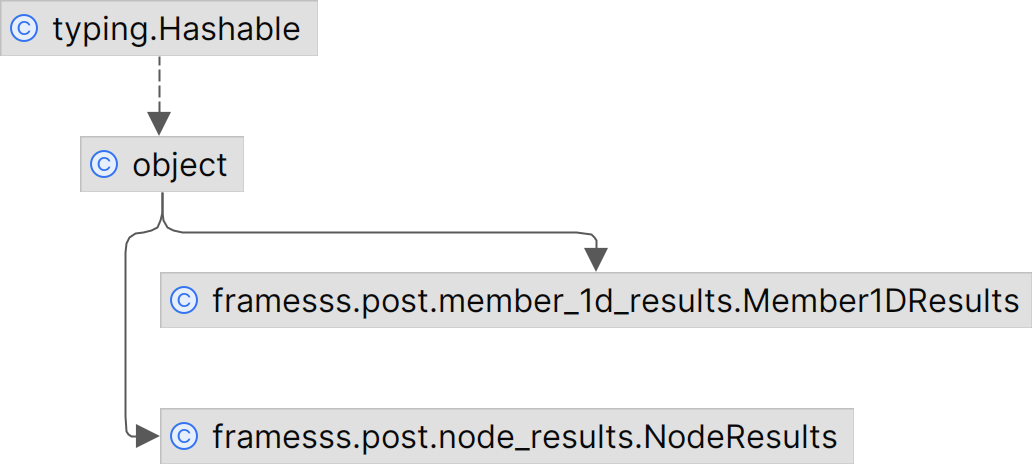
\includegraphics{assets/figures/framesss/uml/post.png}
    \caption{Diagram modulu \texttt{post}}
    \label{fig:modul_post}
\end{figure}
